\section{EXPERIMENTS AND RESULTS}
\label{sec:exps}

\begin{table}[h!]
  \smaller{
  \centering
  \begin{tabular}{|c|c|c|c|c|c|c|}
    \hline
    \textbf{ } & 
    \multicolumn{6}{|c|}{\textbf{Applications}}\\
    \hline
    & Barcelona & Kyoto & San Francisco & Cologne & Lyon & Miami\\
    \hline
    $|V|$ & 13476 & 42456 & 15436 & 56548 & 8174 & 8141 \\
    \hline
    $|E|$ & 25658 & 93722 & 35092 & 115483 & 15586 & 21856 \\
    \hline
  \end{tabular}
  \caption{The task graph setup}
  }
  \label{tab:1}
\end{table}


\begin{figure*}[ht!]
  \centering
  \subfigure[Barcelona]{
    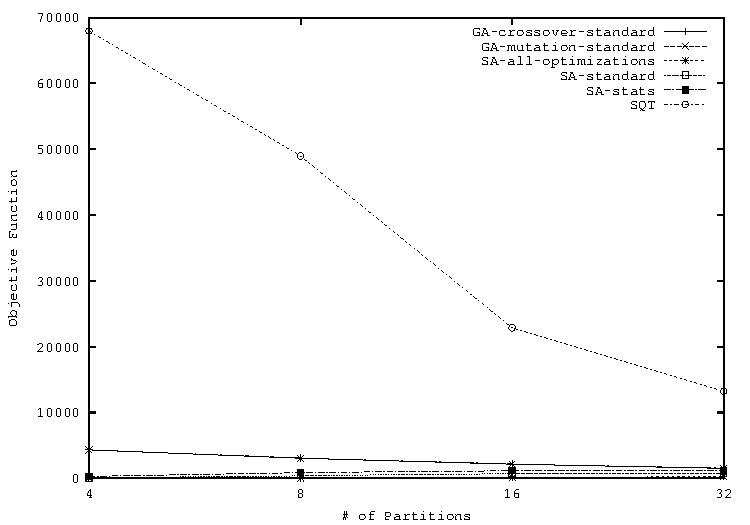
\includegraphics[angle=0, scale=0.4]{./figures/objective1/Barc.pdf}
    \label{fig:obj1barc}
  }
  \subfigure[Kyoto]{
    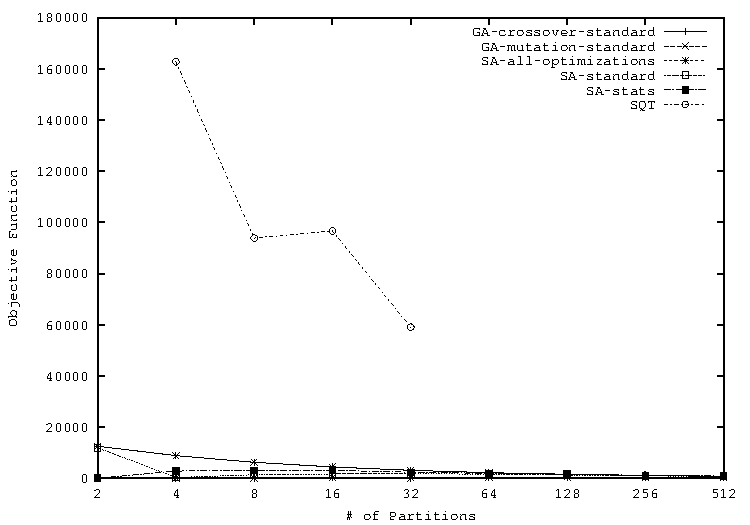
\includegraphics[angle=0, scale=0.4]{./figures/objective1/Kyoto}
    \label{fig:obj1kyoto}
  }
  \subfigure[San Francisco]{
    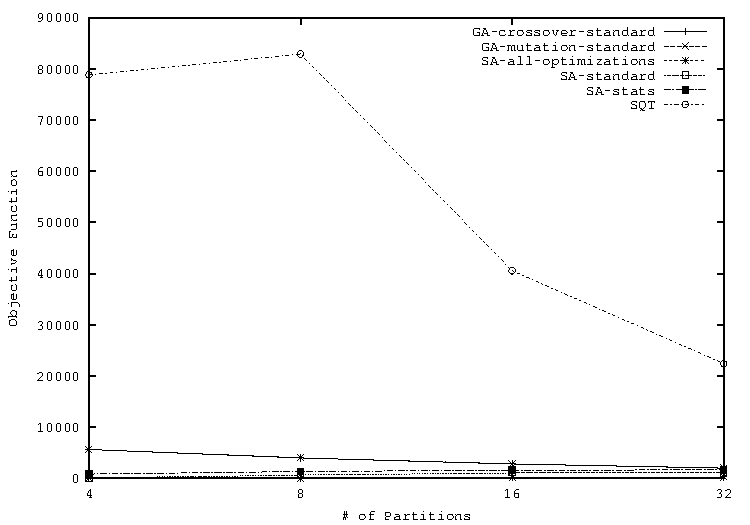
\includegraphics[angle=0, scale=0.4]{./figures/objective1/San}
    \label{fig:obj1san}
  }
  \subfigure[Cologne]{
    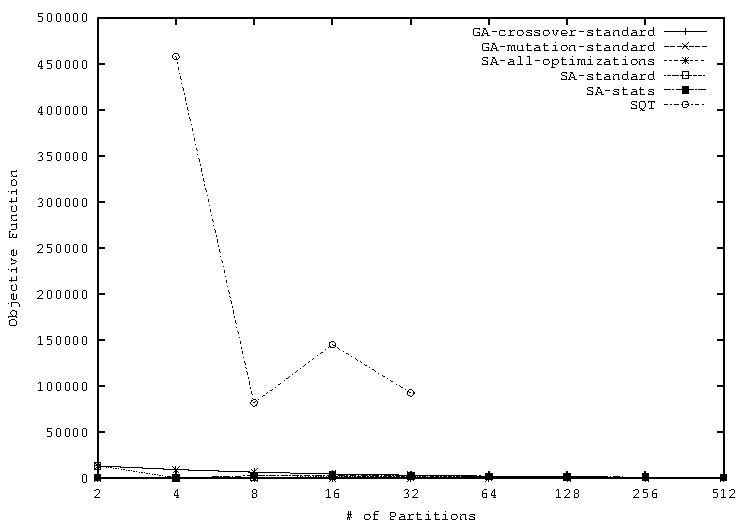
\includegraphics[angle=0, scale=0.4]{./figures/objective1/Cologne}
    \label{fig:obj1cologne}
  }
  \subfigure[Lyon]{
    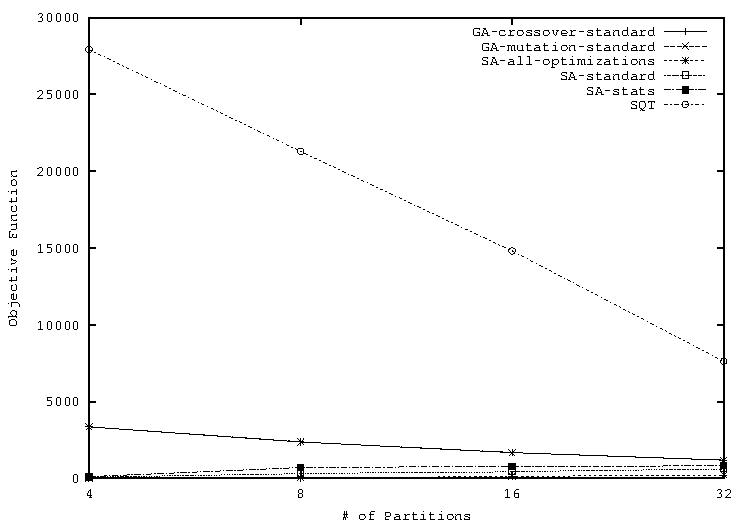
\includegraphics[angle=0, scale=0.4]{./figures/objective1/Lyon}
    \label{fig:obj1lyon}
  }
  \subfigure[Miami]{
    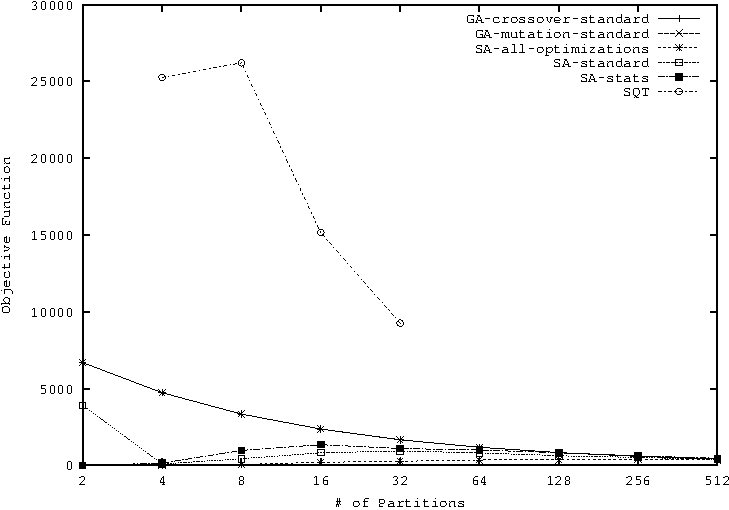
\includegraphics[angle=0, scale=0.4]{./figures/objective1/Miami}
    \label{fig:obj1miami}
  }
  \caption{Comparison of the partioning algorithms based on the first metric(Variance) given by Eq.~\ref{eq:metric3}}
  \label{fig:objective1}
\end{figure*}

\begin{figure*}[t!]
  \centering
  \subfigure[Barcelona]{
    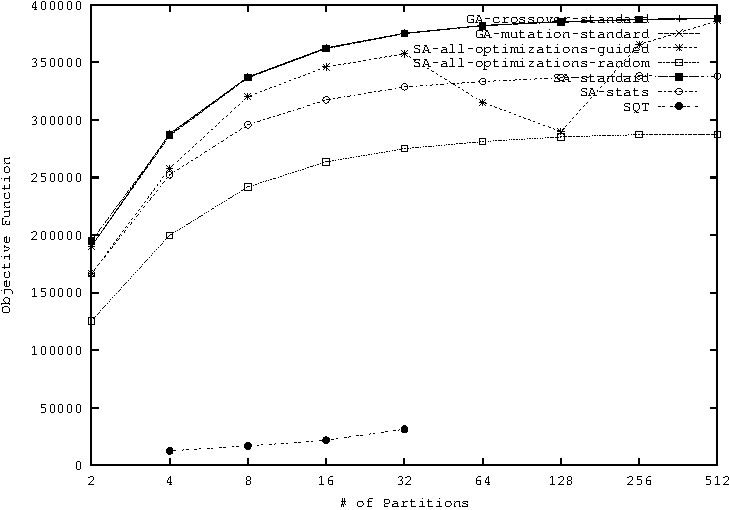
\includegraphics[angle=0, scale=0.4]{./figures/objective2/Barc}
    \label{fig:obj2barc}
  }
  \subfigure[Kyoto]{
    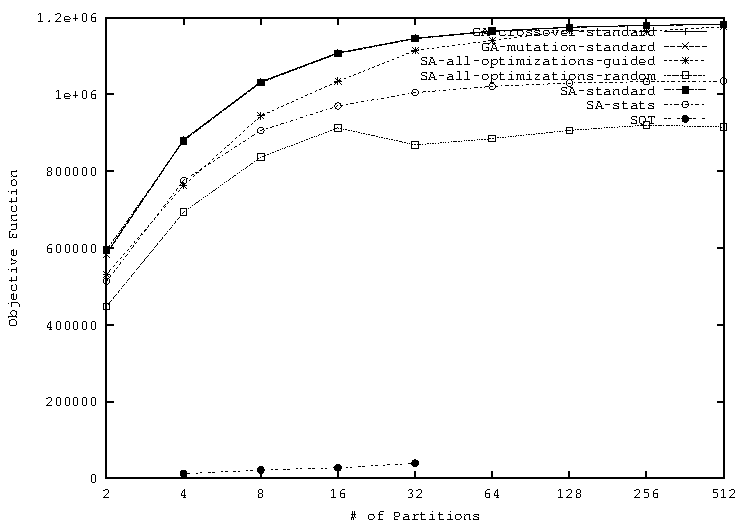
\includegraphics[angle=0, scale=0.4]{./figures/objective2/Kyoto}
    \label{fig:obj2kyoto}
  }
  \subfigure[San Francisco]{
    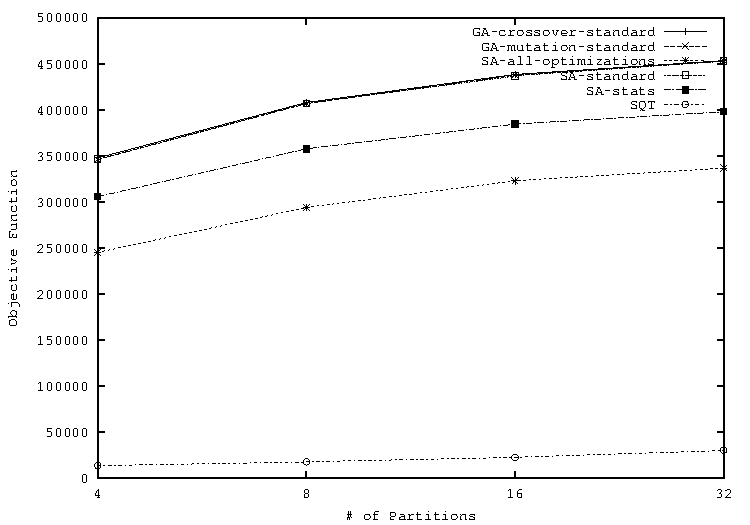
\includegraphics[angle=0, scale=0.4]{./figures/objective2/San}
    \label{fig:obj2san}
  }
  \subfigure[Cologne]{
    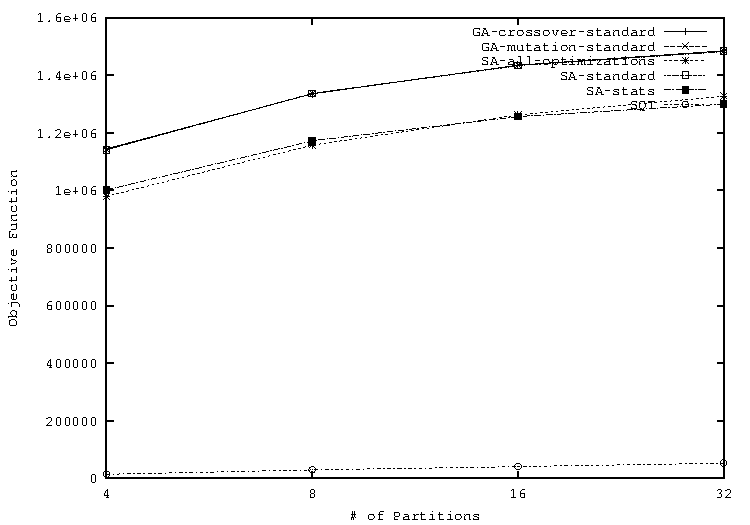
\includegraphics[angle=0, scale=0.4]{./figures/objective2/Cologne}
    \label{fig:obj2cologne}
  }
  \subfigure[Lyon]{
    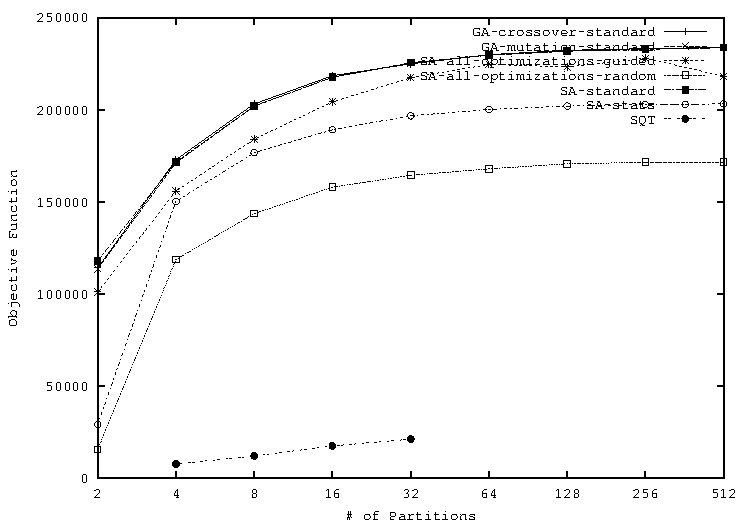
\includegraphics[angle=0, scale=0.4]{./figures/objective2/Lyon}
    \label{fig:obj2lyon}
  }
  \subfigure[Miami]{
    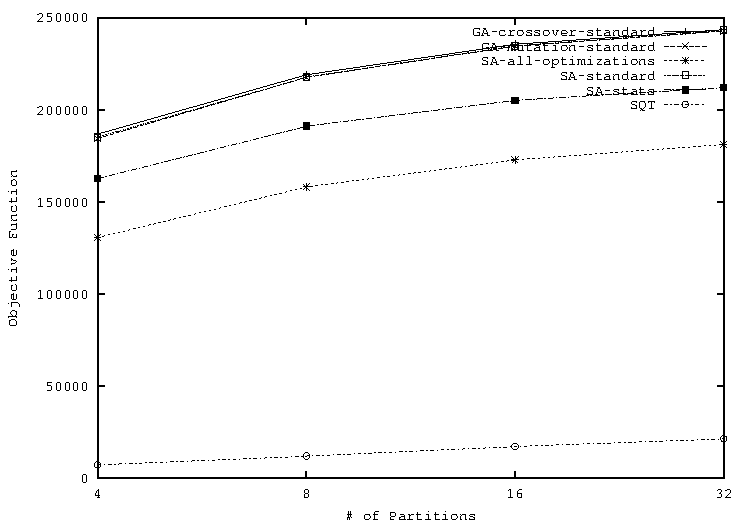
\includegraphics[angle=0, scale=0.4]{./figures/objective2/Miami}
    \label{fig:obj2miami}
  }
  \caption{Comparison of the partitioning algorithms based on the second metric(Inter-Partition Communication) given by Eq.~\ref{eq:metric2}}
  \label{fig:objective2}
\end{figure*}

\begin{figure*}[t!]
  \centering
  \subfigure[Barcelona]{
    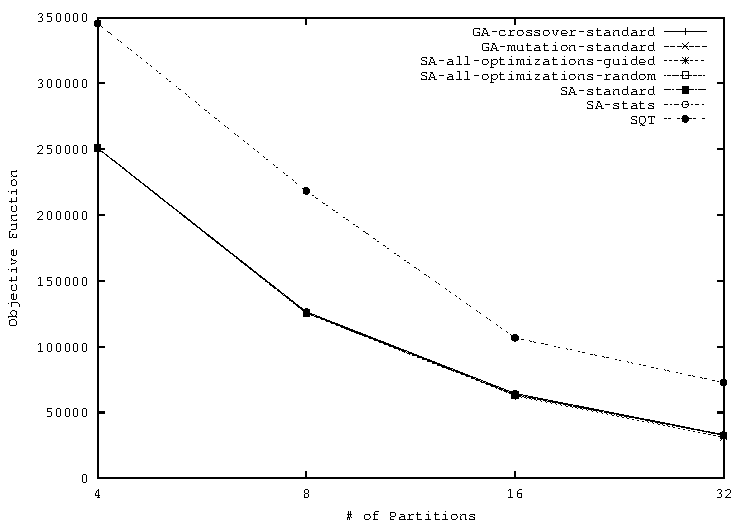
\includegraphics[angle=0, scale=0.4]{./figures/objective3/Barc}
    \label{fig:obj2barc}
  }
  \subfigure[Kyoto]{
    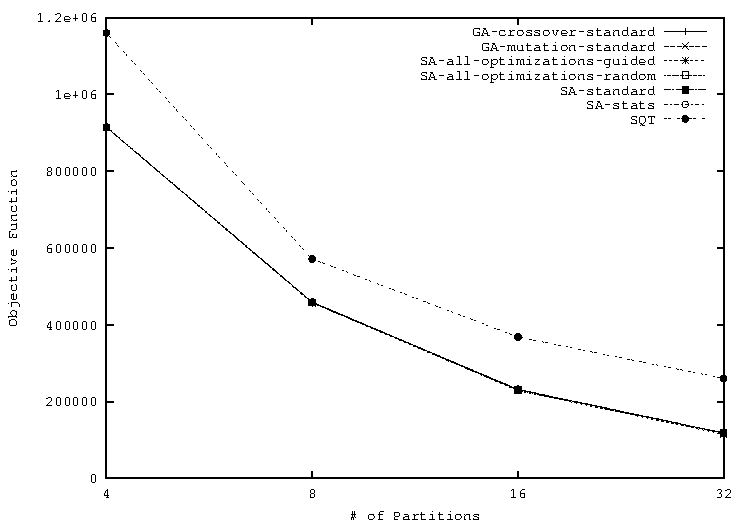
\includegraphics[angle=0, scale=0.4]{./figures/objective3/Kyoto}
    \label{fig:obj2kyoto}
  }
  \subfigure[San Francisco]{
    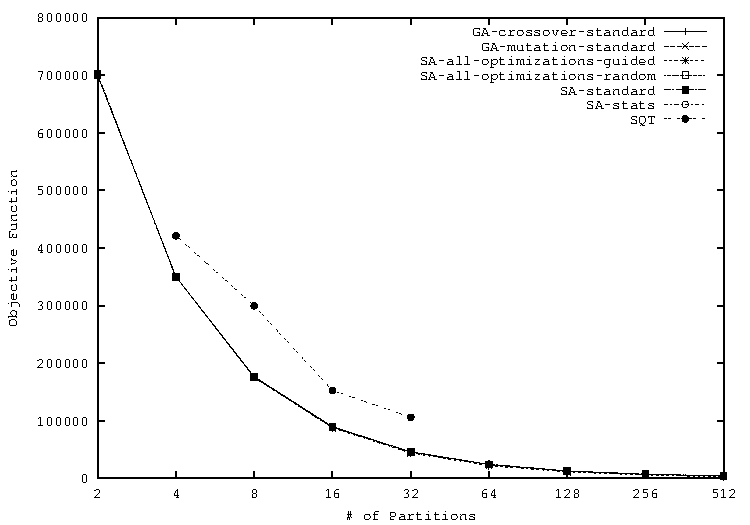
\includegraphics[angle=0, scale=0.4]{./figures/objective3/San}
    \label{fig:obj2san}
  }
  \subfigure[Cologne]{
    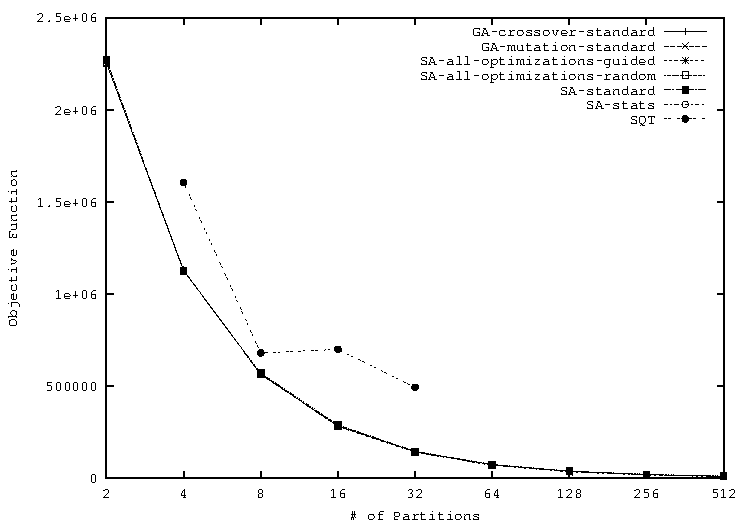
\includegraphics[angle=0, scale=0.4]{./figures/objective3/Cologne}
    \label{fig:obj2cologne}
  }
  \subfigure[Lyon]{
    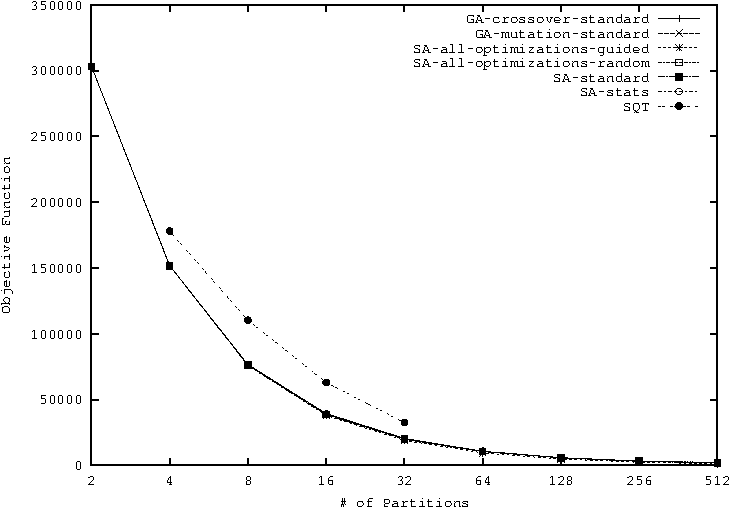
\includegraphics[angle=0, scale=0.4]{./figures/objective3/Lyon}
    \label{fig:obj2lyon}
  }
  \subfigure[Miami]{
    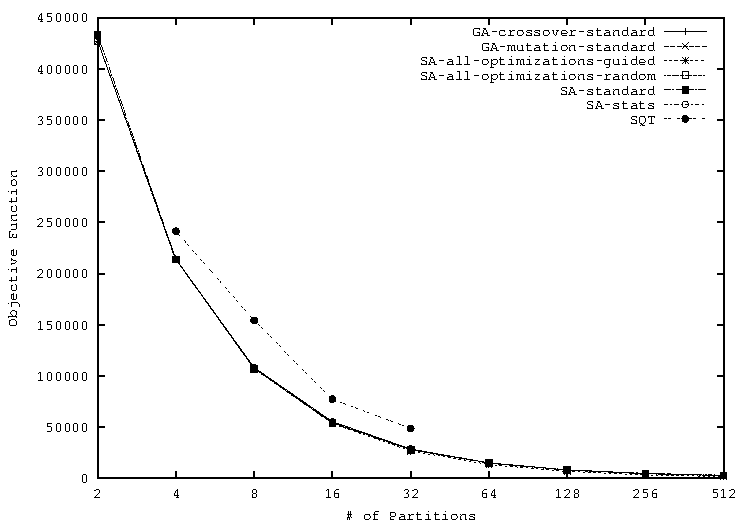
\includegraphics[angle=0, scale=0.4]{./figures/objective3/Miami}
    \label{fig:obj2miami}
  }
  \caption{Comparison of the partitioning algorithms based on the third metric(Max(PartitionSizes)) given by Eq.~\ref{eq:metric1}}
  \label{fig:objective2}
\end{figure*}